\documentclass[10pt,a4paper]{article}
\usepackage[utf8]{inputenc}
\usepackage{amsmath}
\usepackage{amsfonts}
\usepackage{amssymb}
\usepackage{graphicx}
\usepackage{xcolor}
\usepackage{array}
\usepackage{float}
\usepackage{subfig}
\usepackage{parskip}
\usepackage[left=2cm,right=2cm,top=2cm,bottom=2cm]{geometry}
\usepackage{sectsty}
\sectionfont{\usefont{OT1}{phv}{b}{n} \sectionrule{0pt}{0pt}{-5pt}{3pt}}
\author{Songtuan Lin u6162630}
\title{Assignment 1}
\newcolumntype{P}[1]{>{\centering\arraybackslash}p{#1}}
\begin{document}
\maketitle

\section*{Question 1}
For simplicity, I will assume the \textit{HTTP Request} message the server received request a Web Page. 
\begin{figure}[H]
	\center
	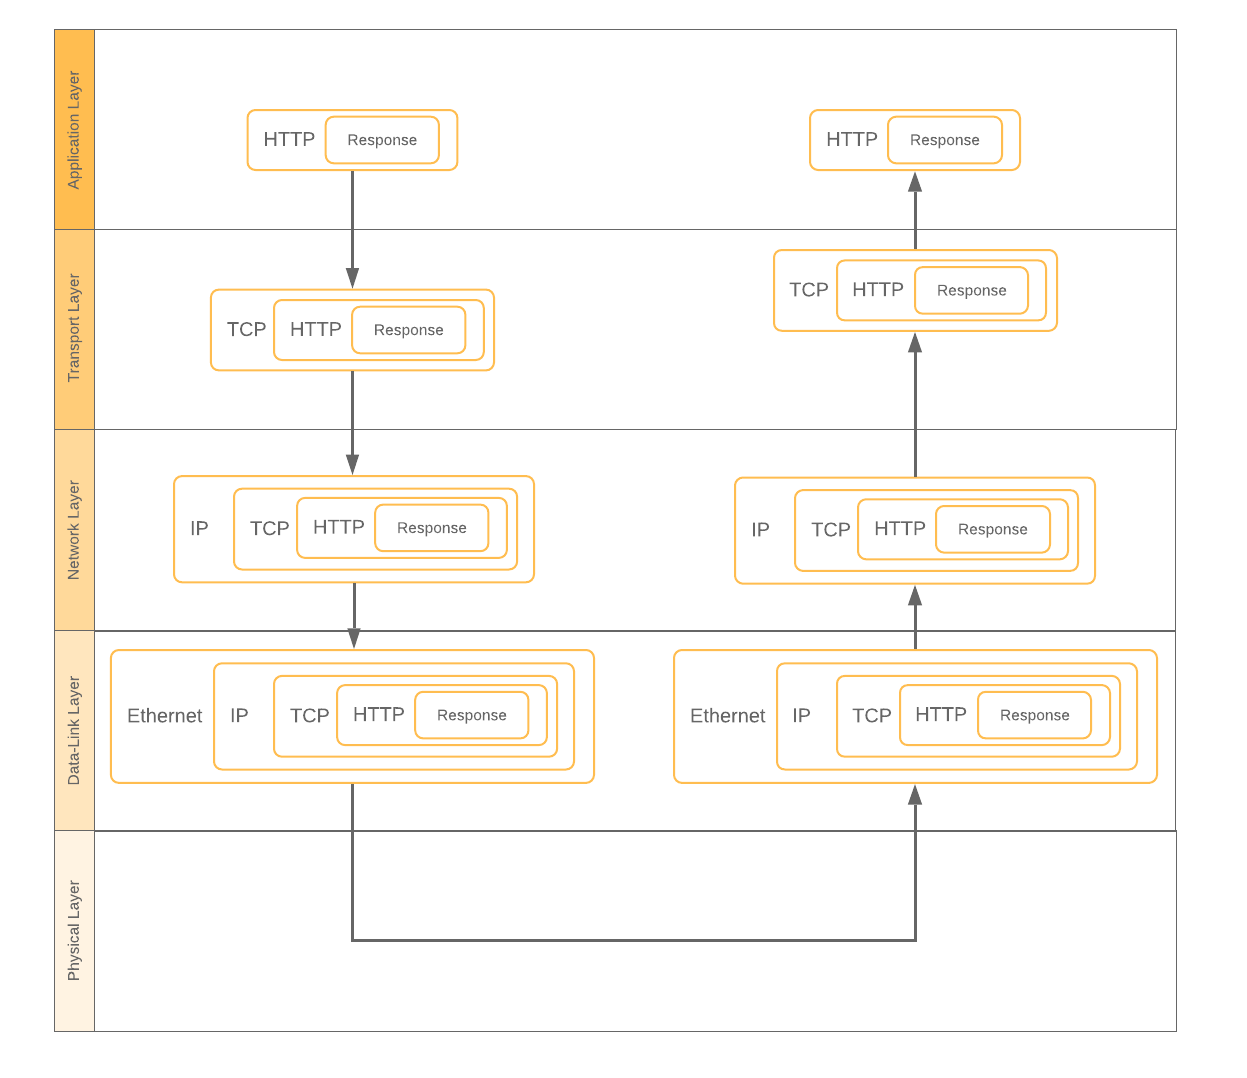
\includegraphics[scale=0.7]{Layers}
	\caption{Transmission through Layers}
	\label{fig_1}
\end{figure}
By comparing Figure \ref{fig_1} with the original Figure, it can be seen that the HTTP Response message will go through the same Network Layer as the HTTP Request message. The only difference shown in these two figures is the \textit{Request} field and \textit{Response} field. Particularity, in this example, the client \textit{request} a Web Page and the server \textit{response} the corresponding html file. Indeed, this simple observation implies a general rule for the communication through computer network:
\begin{quote}
	The message delivery within computer network must go through a series of fixed stages. Each stage will accomplish some specific functions and provide them to be used by another stages.
\end{quote}
Technical, each stage correspond to one Layer, hence, form the modern \textit{Layered-Architecture} as illustrated in Figure \ref{fig_1}. Additionally, in order to maintain the generality of the message within Computer Network, which means the message can be decoded by different host, further rules that specify how each layer accomplish their function have been made. These layer-specific rules are called \textit{protocol}, \textsf{e.g.} HTTP in Application Layer, TCP in Transport Layer, etc. Generally, each protocol need to add some extra information to the original message in order to accomplish their corresponding function. This additional information is called \textit{head}. \textsf{e.g.} HTTP head, TCP head, etc. In the following part, I will briefly explain the function and some common protocols corresponding to each layer:
\begin{itemize}
	\item \textbf{Application Layer}: Application Layer produce the message that will be delivered and transfer it to next Transport Layer. Some popular Application Layer protocols include: HTTP, FTP, etc.
	\item \textbf{Transport Layer}: Transport Layer accomplish the preparation tasks before the delivery, e.g. specify the source and target application of the message, maintain the connection between client and server. The common Transport Layer protocols include: TCP and UDP.
	\item \textbf{Network Layer}: Network Layer determine the route of message delivery, which is one of the most important function. The common Network Layer protocols include OSPF, BGP, etc.
	\item \textbf{Data-Link Layer}: Data-Link Layer further determine the route based on the route calculated by Network Layer. The common protocols in Data-Link Layer include Ethernet, WIFI protocol family, etc.
	\item \textbf{Physical Layer}: Physical Layer is responsible for the actual  transmission.  
\end{itemize}
The above explanation may be too abstract. Indeed, we can think Computer Network as a real world package delivery system, hence, we can have a concrete understand about Layer-Architecture by going through an example: Assume a package delivery company have a package that want to be delivered from Australia to China. The entire delivery process, from Computer Network perspective, can be expressed as:
\begin{enumerate}
	\item The Application Layer get a package from customer that need to be delivered.
	\item The Transport Layer confirm this package delivery order.
	\item The Network Layer determine the route of delivery. Particularly, it determine  which country will be in the delivery path, e.g. Australia $\rightarrow$ Indian $\rightarrow$ China
	\item The Data-Link Layer determine the route that how package will be delivered within country.
	\item The physical Layer carry the package and do the actual transmission.
\end{enumerate}
The above discussion give a theory explanation about Layer-Architecture. Indeed, by using software tools like Wireshark and cURL, we can do some practical experiments to see how Layered-Architecture model work. These practical experiments will be demonstrated in the rest question within .this assignment.

\section*{Question 2}
In this question, I will use cURL to inspect HTTP protocol. This experiment can illustrate the format of HTTP Request and Response message. In order to complete this question, firstly, I need to configure my web server following the setting up instruction described in the question. Particularly, the web server I used is a droplet from Digital-Ocean with IP address: 188.166.167.192. After I have deployed my web server, I can send a HTTP request through cURL by using following command:
\begin{quote}
	\center
	curl -v http://188.166.167.192:8000
\end{quote} 
The output of this cURL command is shown in Figure \ref{co},
\begin{figure}[ht]
	\center
	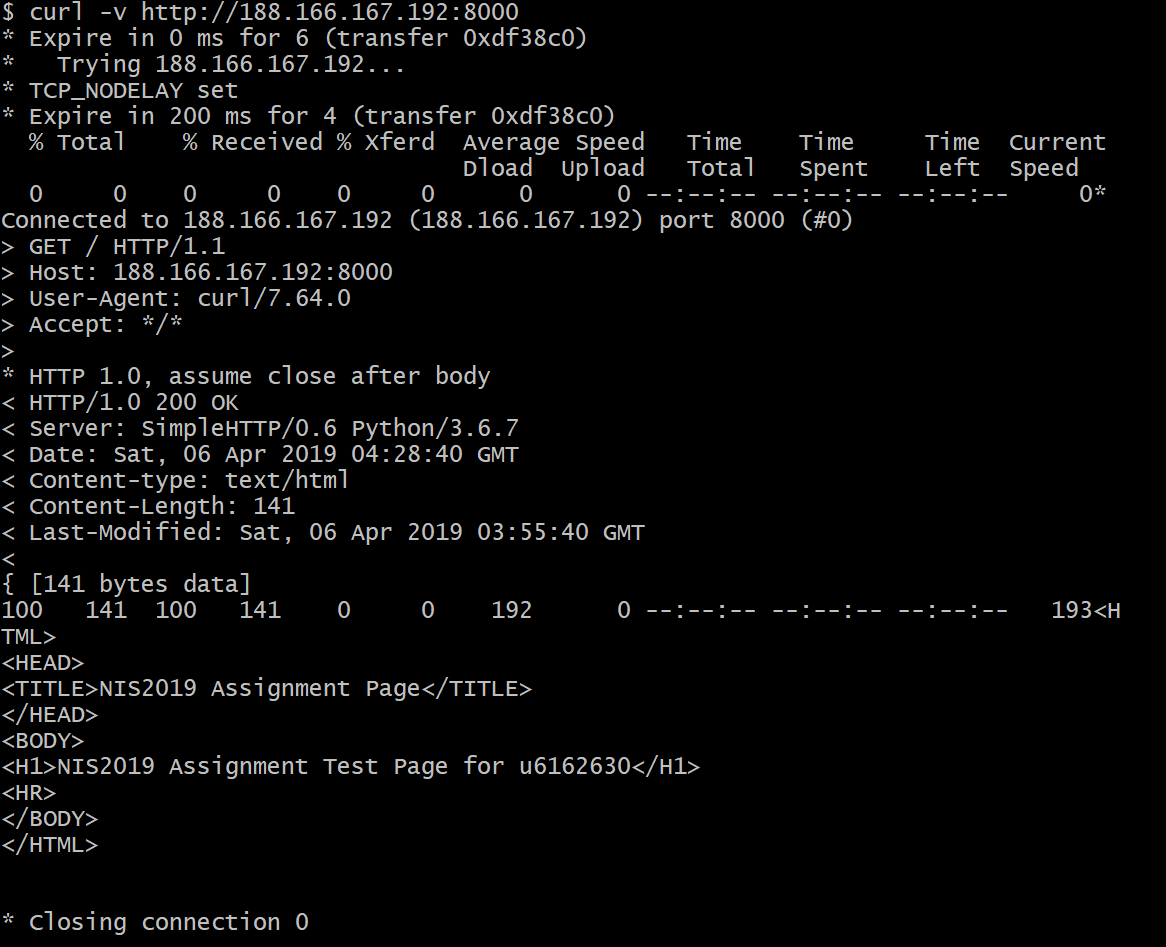
\includegraphics[scale=0.7]{cURL_1}
	\caption{Output of cURL}
	\label{co}
\end{figure}
In which, there are several important content:
\begin{enumerate}
	\item HTTP Request message, which consist of the lines start with '>'. Each line, according to RFC(HTTP), have the following purpose:
		\begin{itemize}
			\item \textbf{Head Line}: This first line specify the request method and the HTTP protocol version. 
			\item \textbf{Host}: Specify the IP address or domain name of the server.
			\item \textbf{User-Agent}: Specify the application that sent this request message along with its' version. In this example, the request is come from  cURL tool.
			\item \textbf{Accept}: Specify the media types which are acceptable for the client. \textsf{i.e.} video stream and audio.
		\end{itemize}
	\item HTTP Response message, which consist of the lines start with '<'. The meaning of each line is:
		\begin{itemize}
			\item \textbf{Head Line}: Serve the same purpose as that in Response message
			\item \textbf{Server}: Specify the server application
			\item \textbf{Date}: The date this response was sent
			\item \textbf{Content-Type}: Specify the file type that this response message will send
			\item \textbf{Content-Length}: Specify the length of the file that will be transformed
			\item \textbf{Last-Modified}: Specify the last date that the file which are willing to be sent is modified.
		\end{itemize}
	\item HTML file, which locate in the last part of the output. This HTML file is the last part of HTTP Response message and correspond to the Web Page requested by clients.
\end{enumerate}
Instead of using cURL to send HTTP Request, we can use simple Web Browser to retrieve the same Web Page, which will be shown in Question 3.

\section*{Question 3}
The HTML file that been created in web server can be retrieved through web browser by typing the following command:
\begin{quote}
	\center
	http://188.166.167.192:8000
\end{quote}
The result that displayed in web browser is:

In this experiment, the web browser send a HTTP Request and receive a HTTP Response from web server. The transmission of HTTP Request and HTTP Response can be illustrated by Figure \ref{fig_1} and follow the general discussion of Layer-Architecture Model in Question 1:
\begin{enumerate}
	\item \textbf{Application Layer}: The web browser in client side(Application) will generate a message called \textit{packet}, which consist of a HTTP head(the definition of head has been given in Question 1) and a request message. This packet will be passed to Transport Layer to have further modification.
	\item \textbf{Transport Layer}: Transport Layer will choose TCP protocol to establish the connection between client and server. Hence, the three-way handshake is required and the TCP head will be added to the original packet.The TCP head append with Application Layer packet is called segment.
	\item \textbf{Network Layer}: Network Layer will calculate the best route for this transmission and add a IP head to the segment, which produce a Network Layer packet.
	\item \textbf{Data-Link Layer}: Data-Link Layer also determine the route, particularly, it determine the transmission route within Local Area Network(LAN). In order to do so, Data-Link Layer need add Ethernet head to Network Layer packet, which produce a frame. 
	\item \textbf{Physical Layer}: Physical Layer take the frame produced by Data-Link Layer and transport it to the server side.
\end{enumerate}
After the server receive the HTTP Request. This message will go through the same Network Layer but in inverse order. Differ from the client side, each Layer in server side will remove the corresponding head. After the sever has processed the request, it will send a HTTP Response through Layer-Architecture Model and reach client. After that, the web browser can finally display the web page.

\end{document}